\chapter{Grundlagen}
Den Begriff Legal Tech trifft man in der heutigen Rechtsbranche immer wieder. Dort ist Legal Tech
ein Trendthema wie künstliche Intelligenz in der IT. Alle diejenigen, die sich am Markt positionieren
wollen, beschäftigen sich mit dem Thema Legal Tech. ,,Definieren kann man Legal Tech als Abkürzung für
den Ausdruck Legal Technology, der die Verbindung von Technologie und Recht im Arbeitsalltag bezeichnet.''\footfullcite[S. 15]{LegalTech}
In diesem Begriff wird die konservative Rechtsbranche mit der progressiven IT- und Technikbranche vereint.
Es wird als das Tool der Zukunft für die Rechtsberatung gehandelt. Anwälte und Richter versprechen sich durch
Legal Tech effizientere, kostengünstigere und konstant qualitativ hochwertige Rechtsberatung und die Möglichkeit, dort rechtliche Unterstützung zu bieten, 
wo es bis jetzt nicht wirtschaftlich sinnvoll war.
Ob durch Legal Robots, Chatbots, Smart Contracts oder einfache digitale Aktenverwaltung: Ziel ist es, alle repetitiven Prozesse
zu automatisieren. Dafür bietet sich das Rechtswesen an, da dort Prozesse zu meist sich wiederholend und immer gleichbleibend sind.
Die Ansprüche sind die selben, die Abläufe sind die selben, lediglich der Mandant ist ein Anderer.

\section{Definiton Legal Tech}
Der Begriff Legal Tech wird in der Branche und in der dazu passenden Literatur verschieden eingesetzt.
Manche meinen mit dem Begriff lediglich das Digitalisieren (Digitisieren) von vorhandenen Prozessen.
Beispielsweise wird der Schriftverkehr nicht mehr per Post, sondern über das besondere elektronische Anwaltspostfach sowohl dem Gericht als auch dem
Gegner zugestellt. Andere wiederum meinen mit Legal Tech die vollautomatisierte Bearbeitung von Rechtsfällen. Um das Ganze
einordnen zu können, hat Oliver Goodenough eine Kategorisierung eingeführt, die es ermöglicht die verschiedenen Ansprüche
an Legal Tech eingliedern zu können. Goodenough kategorisiert Legal Tech in 3 Kategorien: \nameref{Legal Tech 1.0}, \nameref{Legal Tech 2.0}, \nameref{Legal Tech 3.0} \footfullcite{Kategoirien}

\subsection{Legal Tech 1.0} \label{Legal Tech 1.0}
Unter Legal Tech 1.0 (u.a. auch OfficeTech genannt) werden Technologien zusammengefasst, die den im Rechtssektor arbeitenden Menschen den Alltag erleichtern. Es ist die oberste und vermeintlich simpelste Form des Legal Techs. Dazu gehört Aktenverwaltungssoftware, Dokumentenerstellungssoftware und Software zur Unterstützung von Rechtsrecherche. Aber auch Online-Vermarktung, -Recruitment oder -Marktplätze zur Suche von Terminsvertretung (Legal Outsourcing) werden unter dem Begriff Legal Tech 1.0 geführt. Anders ausgedrückt sind es Tools, die wir bereits aus anderen Branchen kennen und für den Rechtssektor angepasst wurden. 
\subsection{Legal Tech 2.0} \label{Legal Tech 2.0}
Legal Tech 2.0 strebt die Ersetzung des menschlichen Juristen innerhalb des bestehenden Systems an. Das soll durch automatisierte Rechtsdienstleistung bewerkstelligt werden. So sollen Programme einzelne Schritte der bestehenden Prozesse übernehmen. Dokumentenauslese, automatische Erstellung juristischer Dokumente, Einordnung der Rechtsansprüche und Erfolgsaussichten, Analyse der Urteile zu einem bestimmten Fall an einem bestimmten Gericht, Vertragserstellung auf Grundlage eines Fragenkataloges an den Mandanten. All dies soll ohne Eingriff eines Juristen erfolgen.

\subsection{Legal Tech 3.0} \label{Legal Tech 3.0}
Legal Tech 3.0 soll das ganze Rechtssystem revolutionieren. Hierbei soll nicht wie in \nameref{Legal Tech 2.0} einzelne Schritte des bestehenden Systems automatisiert werden, sondern das ganze System neu formiert werden. Ziel ist es, komplexe und umfangreiche Rechtsdienstleistungen vollautomatisch abzuschließen. Beispielsweise soll eine autonome Sichtung, Bewertung und auch Verhandlung eines bestimmten Falles ermöglicht werden. Unter diese Kategorie fallen 'Legal Robots / Laywers' oder aber 'Smart Contracts' welche im späteren Verlauf der Arbeit noch genauer beschrieben werden.

\section{Verschiedene Perspektiven auf Legal Tech}
Die von Goodenough eingeführten Kategorien zeigen die Fortschrittlichkeit von Legal Tech an. Dies beschreibt aber leider nur einen Aspekt des Legal Tech's. Waltl, B., Jacob, K. \& Schindler, D haben in Ihrem Artikel ,,Legal Tech – interdisziplinär und kollaborativ'' eine weitere Betrachtungsweise veröffentlicht. Diese Unterteilen Legal Tech auf Sechs verschiedene Perspektiven. Die dazu gelieferte Abbildung soll anschaulich zeigen, aus welchen verschiedenen Aspekten Legal Tech zusammengestellt ist. Abb.\ref{img:Legal Tech – interdisziplinär und kollaborativ}

\begin{figure}
	\centering
	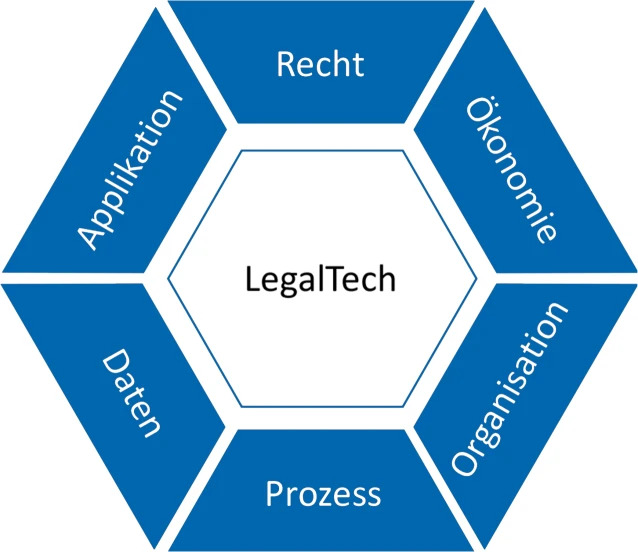
\includegraphics[height=4cm]{Bilder/35764_2020_300_Fig1_HTML.jpg}
	\caption{Zentrale Aspekte von Legal Tech }
	\cite{LegalTechKategorien}
	\label{img:Legal Tech – interdisziplinär und kollaborativ}
\end{figure}

Diese Aspekte bestehen aus 5 Punkten: \footfullcite{LegalTechKategorien}
\subsection{Rechtliche Sicht}
Aus der rechtlichen Sicht muss betrachtet werden, ob ein Einsatz der gegebenen Technologie in diesem bestimmten Gebiet gestattet ist und ob er tatsächlich einen Mehrwert zur Lösung des rechtlichen Problems leistet.

Gerade bei komplexeren oder fachübergreifenden Themen sollte besonders Vorsicht geboten sein. Anwendungen können zu meist nur für rechtliche Themen eingesetzt werden, in denen rechtliche Klarheit besteht. Da die Rechtsprechung in Deutschland nicht einheitlich geregelt ist und Gesetze auslegbar sind, kann es durchaus vorkommen, dass der selbe Rechtsfall an zwei verschiedenen Gerichten unterschiedlich entschieden werden. Hier kommt der Faktor Mensch ins Spiel. Das sollte vor dem Einsatz von Legal Tech zur Unterstützung unbedingt beachtet werden

\subsection{Ökonomische Sicht}
Kann Legal Tech die Effizenz meines Unternehmens erhöhen und gleichzeitig die Risikien minimieren? Kann dadruch ein monetäre Mehrwert entwickelt werden?

Nicht nur der Rechtssektor sondern fast jede Branche setzt auf Optimierung der Prozesse durch technische Unterstützung. Durch den immer steigenden wirtschaftlichen Druck kann ein solcher Vorteil durchaus entscheidend sein. Eine fortschrittliche technische Unterstützung kann das Unternehmen auch für potentielle zukünftige Mitarbeiter attraktiv machen und damit auch einen ökonomischen Vorteil bieten. 

\subsection{Organisationssicht}
Einführung solcher Technologie kann auch eine Veränderung der Organisationsstruktur mit sich führen. Ein Vergleich mit der Einführung eines Enterprise Resource Planning-Systems in Handelsfirmen ist durchaus möglich. Viele Prozesse sollten sich demnach an das System angleichen, um den maximalen Nutzen zu entwickeln. Hierbei ist ein gutes Change Management notwendig \footfullcite{LegalTech}. Dabei sollte darauf geachtet werde, dass die Personen, deren Aufgaben durch die neue Technologie erledigt werden, eine andere passende Aufgabe erhalten. Das erhöht die Akzeptanz der Technik unter den Mitarbeitern


\subsection{Prozesssicht}
Welche Prozesse sollen von Legal Tech unterstützt werden?

Um diese Frage zu beantworten, müssen zunächst die Abläufe und Prozesse genaustens festgelegt und modelliert werden. Erst dann ist eine zuverlässige Beantwortung dieser Frage möglich. 

\subsection{Applikationssicht}
Welche Aufgaben sollen von der Technologie erledigt werden und können diese von bestehenden Anwendungen erfüllt werden oder müssen neue Anwendungen entwickelt zur Verfügung gestellt werden.

\subsection{Datensicht}
Datensicht: Liegen notwendige Daten vor oder können und dürfen diese erhoben, verarbeitet und gespeichert werden, damit die Technologie ihr volles Potenzial entfalten kann?

Alle Applikationen im Legal Tech brauchen in einer Weise Daten. Ohne Daten kann kein mehr wert geschaffen werden. Diese Daten müssen dann auch zwischen verschiedenen Anwendungen verteilt werden können. Daher ist es wichtig, dass im Legal Tech-Sektor nicht nur auf die Datenmasse und Integretät geachtet wird, sondern selbstverständlich auch auf die rechtlichen Grundlagen dafür.